\section{Performance and Visual Results}\label{sec:performance_visual_results}

% Bad performance, not optimized, visually not that conviencing because of bad
% parameters and which have to be guessed, brdf and fresnel problem. No opinion
% yet.

We tested our application on a MacBook Pro Retina (Late 2013) with an Intel i7
2.8 GHz processor and an integrated Intel Iris 1.5 GB graphic card. The
application ran on an external monitor having the resolution of 1920$\times$1080
pixels. The application itself ran in 800$\times$600 window. The number of
vertices used to represent the water was 900. The average computation time of a
frame was 58.8978ms.

The results of our implementation can be seen in \autoref{fig:application} on
page~\pageref{fig:application}.  \autoref{fig:reference} on
page~\pageref{fig:reference} shows our reference images.

\begin{figure}[htb!]
    \centering
    \begin{subfigure}[htb!]{\textwidth}
        \centering
        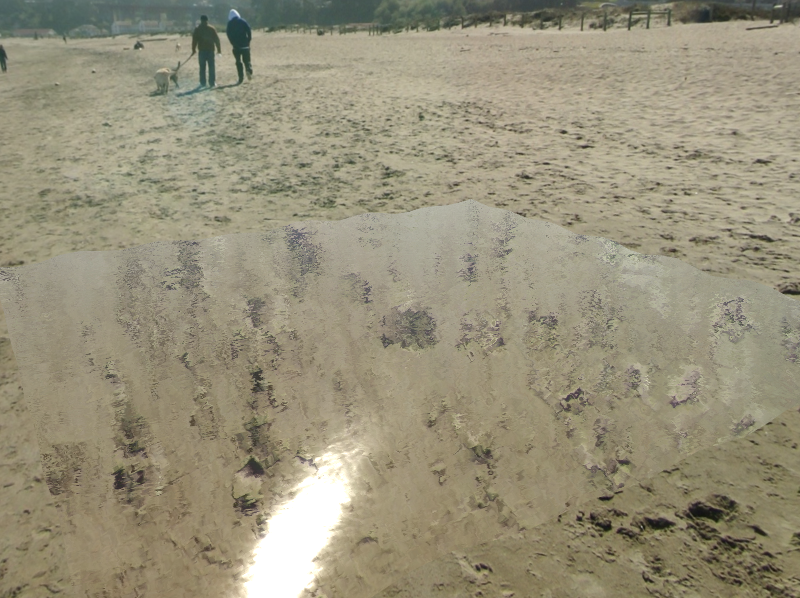
\includegraphics[height=7cm]{application_1.png}\label{fig:application_1}
    \end{subfigure}\\
    %  
    \begin{subfigure}[htb!]{\textwidth}
        \centering
        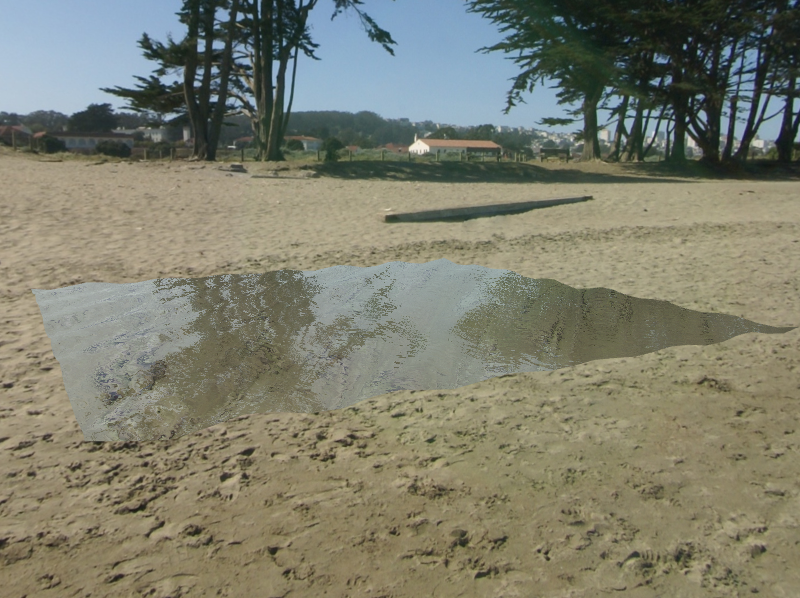
\includegraphics[height=7cm]{application_2.png}\label{fig:application_2}
    \end{subfigure}
\end{figure}
\begin{figure}[htb!]\ContinuedFloat{}
    \centering
    \begin{subfigure}[htb!]{\textwidth}
        \centering
        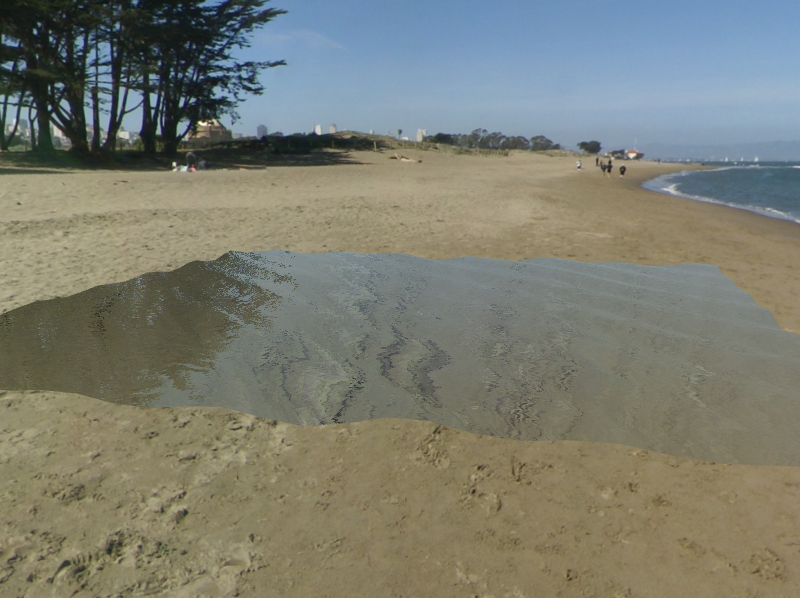
\includegraphics[height=7cm]{application_3.png}\label{fig:application_3}
    \end{subfigure}\\
    %  
    \begin{subfigure}[htb!]{\textwidth}
        \centering
        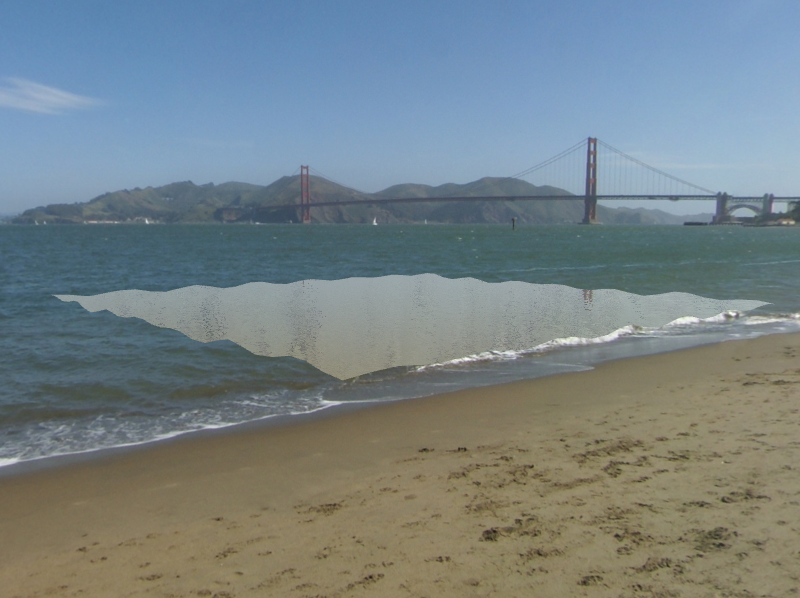
\includegraphics[height=7cm]{application_4.png}\label{fig:application_4}
    \end{subfigure}
    \caption{Result of our implementation}\label{fig:application}
\end{figure}


\begin{figure}[htb!]
    \centering
    \begin{subfigure}[htb!]{\textwidth}
        \centering
        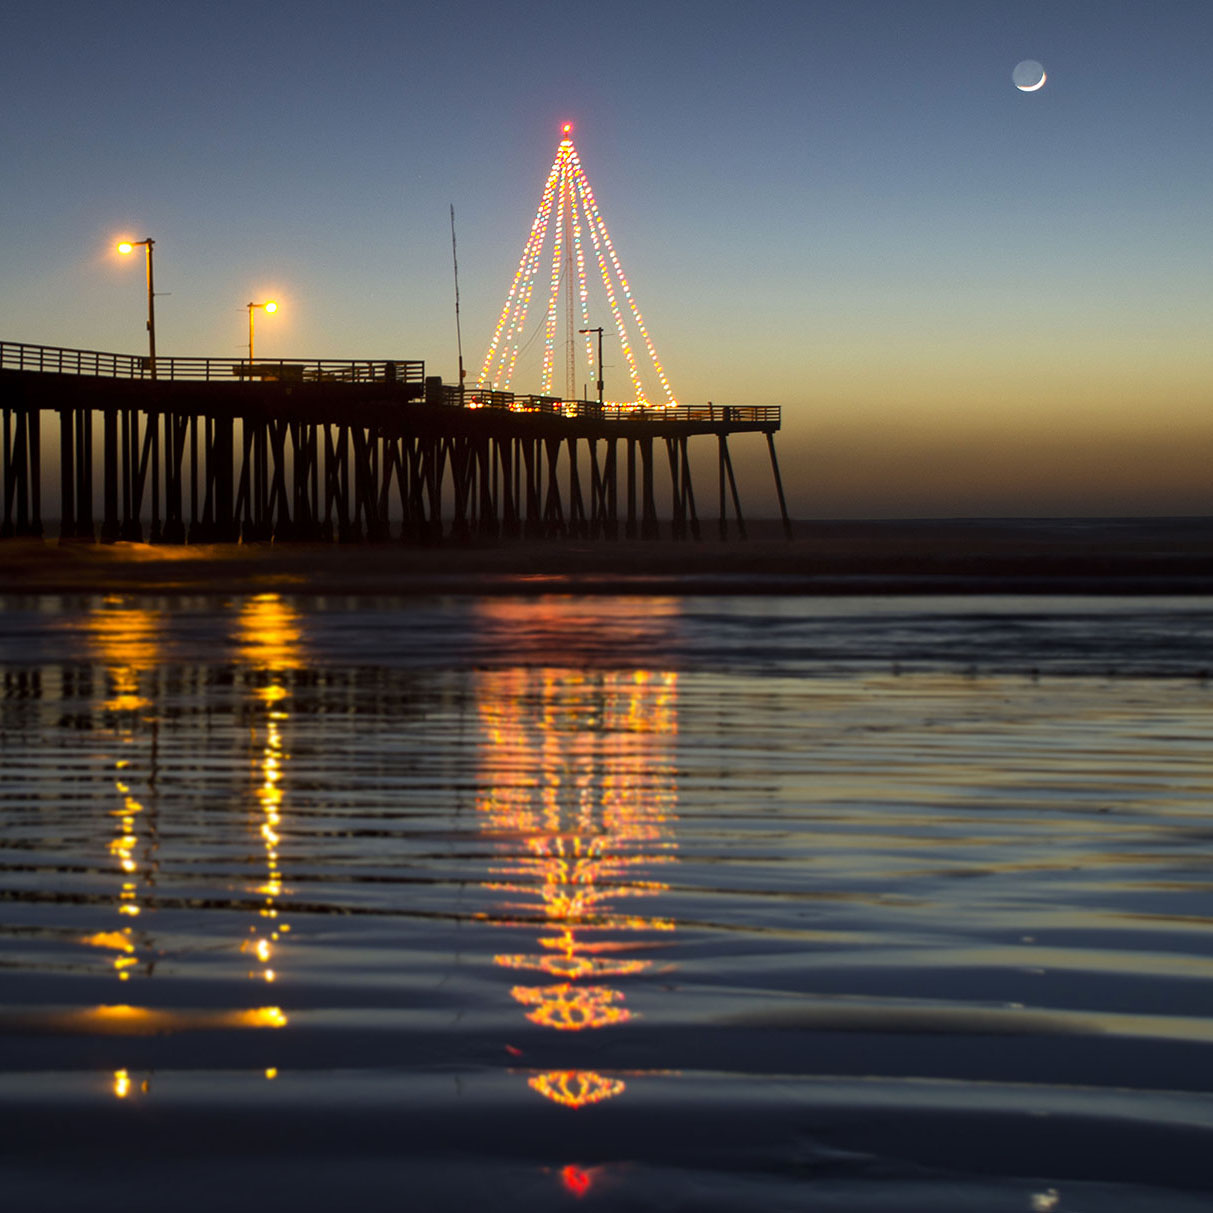
\includegraphics[height=9cm]{reference_1.jpg}\label{fig:reference_1}
    \end{subfigure}\\
    %  
    \begin{subfigure}[htb!]{\textwidth}
        \centering
        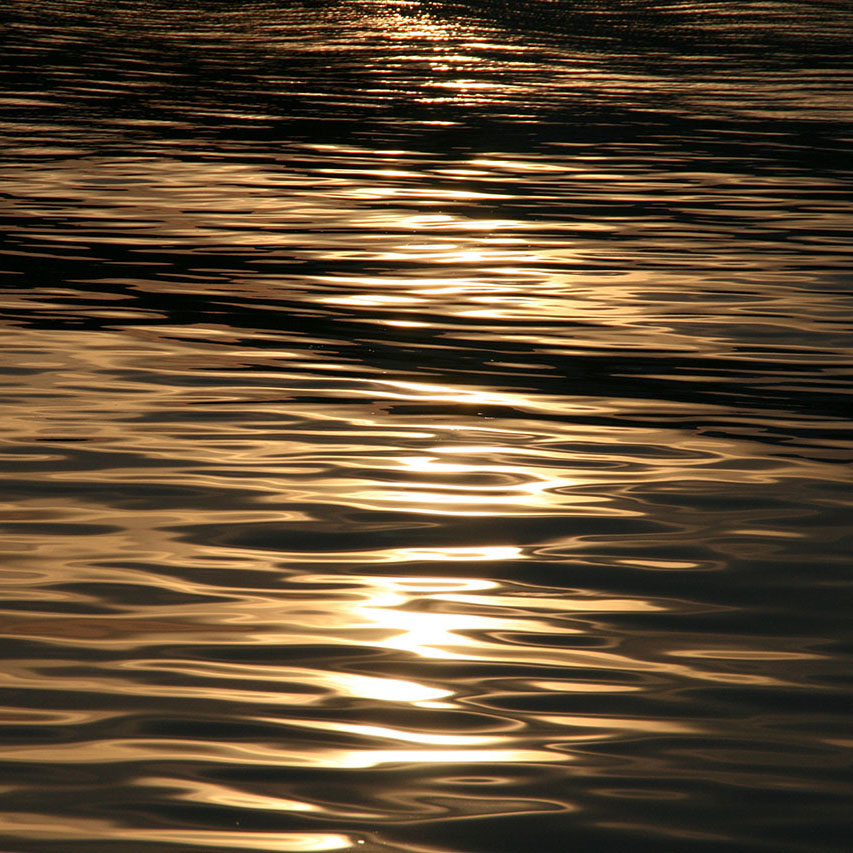
\includegraphics[height=9cm]{reference_2.jpg}\label{fig:reference_2}
    \end{subfigure}
    \caption{Reference images}\label{fig:reference}
\end{figure}
